%\documentclass[tikz,convert={outfile=\jobname.svg}]{standalone}
\documentclass[10pt,landscape]{article}

\usepackage[T1]{fontenc}
\usepackage{lmodern}
\usepackage{tikz}

\definecolor{dark1}{HTML}{E41A1C}
\definecolor{dark2}{HTML}{377Eb8}
\definecolor{dark3}{HTML}{4DAF4A}
\definecolor{dark4}{HTML}{984EA3}
\definecolor{A1}{HTML}{1b9e77}
\definecolor{A2}{HTML}{d95f02}

\definecolor{R1}{HTML}{fee0d2}
\definecolor{R2}{HTML}{fc9272}
\definecolor{R3}{HTML}{de2d26}

\pagestyle{empty}
\begin{document}
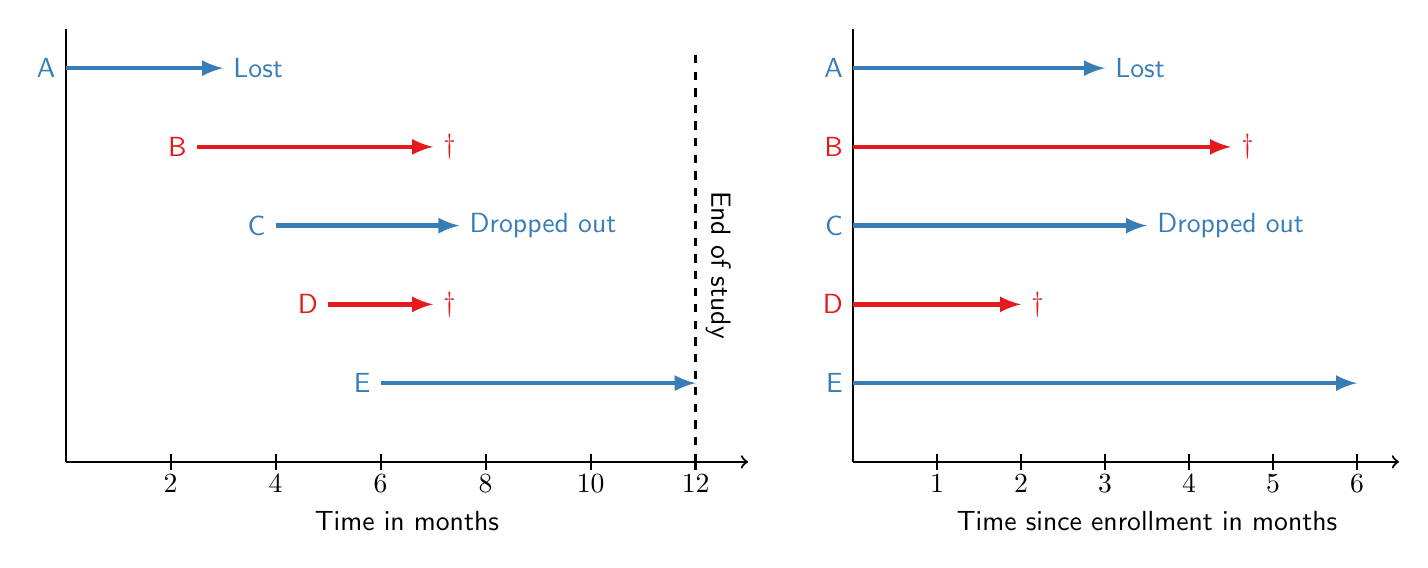
\begin{tikzpicture}[yscale=1.0,xscale=1.33333,font=\sffamily]
\begin{scope}[thick]
% Axes:
\draw [->] (0,0) -- (6.5,0);
\draw [-] (0,0) -- (0,5.5);
\draw [dashed] (6,0) -- (6,5.25);

% Axes labels:
\foreach \n in {1,...,6}{%
    \pgfmathparse{int(\n * 2)}
    \edef\v{\pgfmathresult}
    \draw (\n,-3pt) -- (\n,3pt) node [below,yshift=-4pt] {$\v$};
}
\end{scope}

\begin{scope}[thick]
\node [below,align=center] at (+3.25,-0.5) {Time in months};

\node [rotate=-90,above] at (6,2.5) {End of study};

% Start and end points
\node [left,dark2] (start_a) at (+0, 5) {A};
\node [right,dark2] (end_a) at (+1.5, 5) {Lost};

\node [left,dark1] (start_b) at (+1.25, 4) {B};
\node [right,dark1] (end_b) at (+3.5, 4) {$\dagger$};

\node [left,dark2] (start_c) at (+2, 3) {C};
\node [right,dark2] (end_c) at (+3.75, 3) {Dropped out};

\node [left,dark1] (start_d) at (+2.5, 2) {D};
\node [right,dark1] (end_d) at (+3.5, 2) {$\dagger$};

\node [left,dark2] (start_e) at (+3, 1) {E};
\node [right,dark2] (end_e) at (+6, 1) {};
\end{scope}

% Lines connecting start and end
\begin{scope}[ultra thick,every path/.style={draw, -latex}]
\path[dark2] (start_a) -- (end_a);
\path[dark1] (start_b) -- (end_b);
\path[dark2] (start_c) -- (end_c);
\path[dark1] (start_d) -- (end_d);
\path[dark2] (start_e) -- (end_e);
\end{scope}

%%%
%% RIGHT
%%%
\begin{scope}[xshift=7.5cm,xscale=.8]
\begin{scope}[thick]
% Axes:
\draw [->] (0,0) -- (6.5,0);
\draw [-] (0,0) -- (0,5.5);

% Axes labels:
\foreach \n in {1,...,6}{%
    \draw (\n,-3pt) -- (\n,3pt) node [below,yshift=-4pt] {$\n$};
}
\end{scope}

\begin{scope}[thick]
\node [below,align=center] at (+3.5,-0.5) {Time since enrollment in months};

% Start and end points
\node [left,dark2] (start_a2) at (0, 5) {A};
\node [right,dark2] (end_a2) at (+3, 5) {Lost};

\node [left,dark1] (start_b2) at (0, 4) {B};
\node [right,dark1] (end_b2) at (+4.5, 4) {$\dagger$};

\node [left,dark2] (start_c2) at (0, 3) {C};
\node [right,dark2] (end_c2) at (+3.5, 3) {Dropped out};

\node [left,dark1] (start_d2) at (0, 2) {D};
\node [right,dark1] (end_d2) at (+2, 2) {$\dagger$};

\node [left,dark2] (start_e2) at (0, 1) {E};
\node [right,dark2] (end_e2) at (+6, 1) {};
\end{scope}

% Lines connecting start and end
\begin{scope}[ultra thick,every path/.style={draw, -latex}]
\path[dark2] (start_a2) -- (end_a2);
\path[dark1] (start_b2) -- (end_b2);
\path[dark2] (start_c2) -- (end_c2);
\path[dark1] (start_d2) -- (end_d2);
\path[dark2] (start_e2) -- (end_e2);
\end{scope}
\end{scope}
\end{tikzpicture}
\end{document}